\documentclass[10pt,a4paper,twoside]{article}
\usepackage[T1]{fontenc}
\usepackage{booktabs}
\usepackage{amsfonts,amssymb,amsmath}
\usepackage{tikz}
\usepackage{multirow}
\usepackage{fourier}
\title{Species Classifier Design Space Exploration}
\author{Munim Zabidi}
\begin{document}
	\maketitle
% ==============================================================================
% Model Evolution Narrative - From Baseline to State-of-the-Art
% For Q1 Publication Submission
% ==============================================================================

\section{Model Architecture Evolution}
\label{sec:evolution}

This section chronicles the systematic exploration of neural architectures for resource-constrained avian acoustic classification, documenting the progression from established computer vision baselines through audio-specific adaptations to the final optimized architecture.

% ==============================================================================
\subsection{Phase 1: Computer Vision Baselines}
\label{sec:phase1}

\subsubsection{Initial Exploration: MobileNetV3-Small}

We began with MobileNetV3-Small~\cite{howard2019searching}, a proven architecture for edge deployment, adapting it for mel-spectrogram classification (Table~\ref{tab:mobilenet_baseline}).

\begin{table}[h]
	\centering
	\caption{MobileNetV3-Small Baseline Results (64$\times$300 input)}
	\label{tab:mobilenet_baseline}
	\begin{tabular}{lcccc}
		\toprule
		\textbf{Variant} & \textbf{Params} & \textbf{Size (KB)} & \textbf{FP32 Acc.} & \textbf{INT8 Acc.} \\
		\midrule
		Original (width=1.0) & 2.54M & 2,478 & 94.44\% & 93.56\% \\
		Width multiplier 0.75 & 1.53M & 1,495 & 94.11\% & 93.11\% \\
		Width multiplier 0.5 & 0.72M & 703 & 92.78\% & 91.67\% \\
		Width multiplier 0.35 & 0.39M & 381 & 90.44\% & 89.11\% \\
		\bottomrule
	\end{tabular}
\end{table}

\noindent\textbf{Key Findings:}
\begin{itemize}
	\item Width multiplier 0.75 achieved best accuracy-size trade-off (93.11\%, 1.5M params)
	\item Post-training quantization (PTQ) incurred 0.88--1.33\% accuracy degradation
	\item All variants exceeded target 512~KB deployment constraint
	\item Architecture designed for spatial vision tasks, not optimized for temporal-spectral patterns
\end{itemize}

\subsubsection{Limitations of Vision-Centric Architectures}

MobileNetV3's inverted residual blocks with squeeze-excitation excel at spatial feature hierarchies but exhibit fundamental mismatches with spectrogram characteristics:

\begin{enumerate}
	\item \textbf{Isotropic convolutions}: Treat frequency and time dimensions equivalently, ignoring distinct mel-scale frequency structure versus linear time progression
	\item \textbf{Aggressive downsampling}: Early stride-2 convolutions discard fine-grained temporal detail critical for distinguishing similar vocalizations
	\item \textbf{Squeeze-excitation bias}: Channel attention optimized for RGB channels, not spectro-temporal feature maps
	\item \textbf{Parameter inefficiency}: Dense pointwise convolutions consume excessive memory for marginal gains on sequential patterns
\end{enumerate}

These observations motivated exploration of audio-aware architectures.

% ==============================================================================
\subsection{Phase 2: Audio-Focused Adaptations}
\label{sec:phase2}

\subsubsection{Depthwise-Separable CNN (DS-CNN)}

Inspired by speech command recognition~\cite{zhang2017hello}, we adopted DS-CNN as a lightweight baseline tailored for spectro-temporal patterns (Table~\ref{tab:dscnn_evolution}).

\begin{table}[h]
	\centering\small
	\caption{DS-CNN Architecture Evolution}
	\label{tab:dscnn_evolution}
	\begin{tabular}{lcccl}
		\toprule
		\textbf{Model} & \textbf{Params} & \textbf{Size (KB)} & \textbf{INT8 Acc.} & \textbf{Key Innovation} \\
		\midrule
		1a: DS-CNN Baseline & 194K & 189 & 91.67\% & Depthwise-separable blocks \\
		1b: + Wider Initial & 297K & 290 & 92.89\% & 64-channel stem \\
		1c: + Squeeze-Excite & 318K & 311 & 93.56\% & Channel attention \\
		1d: + Residual + Attn. & 309K & 302 & 94.22\% & Skip + MHSA \\
		\midrule
		\textit{1e: Final (Ours)} & \textit{462K} & \textit{451} & \textit{\textbf{95.67\%}} & \textit{Residual-all + 80 mels} \\
		\bottomrule
	\end{tabular}
\end{table}

\noindent\textbf{Architectural Components:}

\begin{enumerate}
	\item \textbf{Depthwise-Separable Convolution:} Factorizes standard 3$\times$3 convolution into:
	\begin{itemize}
		\item Depthwise: Per-channel 3$\times$3 spatial filtering (720 params for 80 channels)
		\item Pointwise: 1$\times$1 cross-channel mixing (6,400 params for 80$\to$80)
		\item \textit{Result:} 8.9$\times$ parameter reduction vs. standard convolution
	\end{itemize}

	\item \textbf{Squeeze-and-Excitation (SE):} Lightweight channel attention~\cite{hu2018squeeze}
	\begin{equation}
		\text{SE}(x) = x \odot \sigma\left(W_2 \, \text{ReLU}(W_1 \, \text{GAP}(x))\right)
	\end{equation}
	where GAP = global average pooling, $r$ = reduction ratio (8--24), adding $2 \times C^2/r$ parameters per block.

	\item \textbf{Residual Connections:} Introduced in all four DS blocks:
	\begin{equation}
		y = \text{ReLU}\left(\text{SE}(\text{DSConv}(x)) + \mathcal{P}(x)\right)
	\end{equation}
	where $\mathcal{P}(x)$ applies 1$\times$1 projection if input/output channels differ.

	\item \textbf{Lightweight Multi-Head Self-Attention (MHSA):} Applied after final DS block:
	\begin{equation}
		\text{MHSA}(X) = \text{Concat}(\text{head}_1, \ldots, \text{head}_h) W^O
	\end{equation}
	with $h=2$ heads, $d_k=32$ key dimension, and attention over 90 temporal-frequency patches (5$\times$18 after pooling).
\end{enumerate}

\noindent\textbf{Progressive Improvements:}
\begin{itemize}
	\item \textit{Model 1a $\to$ 1b (+1.22\%):} Wider 64-channel stem captures richer initial features, enabling residual skip in first block
	\item \textit{Model 1b $\to$ 1c (+0.67\%):} SE blocks recalibrate channel importance, suppressing noise-dominated bands
	\item \textit{Model 1c $\to$ 1d (+0.66\%):} Residual connections improve gradient flow; MHSA captures long-range temporal dependencies (e.g., trill patterns)
	\item \textit{Model 1d $\to$ 1e (+1.45\%):} Residual in all blocks + 80 mel bins (vs. 64) increase capacity while staying within budget
\end{itemize}

\subsubsection{Why DS-CNN Outperforms MobileNetV3}

Compared to MobileNetV3-Small (width 0.5: 703~KB, 91.67\%), our DS-CNN 1e achieves:
\begin{itemize}
	\item \textbf{+3.9\% accuracy} (95.67\% vs. 91.67\%)
	\item \textbf{35\% smaller} (451~KB vs. 703~KB)
	\item \textbf{Simpler architecture}: 4 uniform DS blocks vs. 11 heterogeneous inverted residual blocks
\end{itemize}

\noindent\textit{Root cause:} DS-CNN's inductive bias aligns with spectrogram structure—depthwise operations naturally separate spectral and temporal processing, while MobileNetV3's inverted bottlenecks waste capacity on vision-specific priors (e.g., receptive field expansion for object recognition).

% ==============================================================================
\subsection{Phase 3: Temporal Convolutional Networks (TCN)}
\label{sec:phase3}

Motivated by sequence modeling successes~\cite{bai2018empirical}, we explored Temporal Convolutional Networks (TCN) as an alternative to recurrent architectures for capturing long-range temporal dependencies without RNN overhead.

\subsubsection{TCN Architecture Principles}

TCNs employ:
\begin{enumerate}
	\item \textbf{Causal dilated convolutions}: Exponentially expanding receptive fields
	\begin{equation}
		\text{RF} = 1 + 2 \sum_{i=0}^{L-1} (k-1) \cdot 2^i
	\end{equation}
	where $k$ = kernel size, $L$ = layers. For $k=3$, $L=8$: RF = 511 frames (5.1 seconds).

	\item \textbf{Residual blocks}: Skip connections stabilize deep temporal stacks

	\item \textbf{1D convolutions}: Process pre-pooled spectrogram embeddings (after Conv2D stem)
\end{enumerate}

\subsubsection{Systematic TCN Ablation Study}

We conducted seven controlled experiments to isolate TCN design factors (Table~\ref{tab:tcn_ablation}).

\begin{table}[h]
	\centering
	\caption{TCN Ablation Study (64$\times$300 input, Mixup $\alpha=0.2$)}
	\label{tab:tcn_ablation}
	\begin{tabular}{lcccc}
		\toprule
		\textbf{Variant} & \textbf{Params} & \textbf{Size (KB)} & \textbf{INT8 Acc.} & \textbf{Modification} \\
		\midrule
		4a: Baseline (8 layers) & 242K & 236 & 92.00\% & Dilation [1,2,4,8,16,32,64,128] \\
		4b: Shallow (4 layers) & 162K & 158 & 91.33\% & Dilation [1,2,4,8] \\
		4c: Wide (128 channels) & 461K & 450 & 92.44\% & 2$\times$ channel width \\
		4d: Deep (10 layers) & 298K & 291 & 92.22\% & +2 layers, dilation to 512 \\
		4e: Kernel-2 & 194K & 189 & 91.56\% & $k=2$ (receptive field = 255) \\
		4f: Kernel-5 & 337K & 329 & 92.11\% & $k=5$ (receptive field = 1,023) \\
		4g: No-residual & 242K & 236 & 90.89\% & Removed skip connections \\
		4h: Lightweight & 142K & 139 & 90.67\% & 32 channels, 6 layers \\
		\midrule
		\textit{DS-CNN 1e (ours)} & \textit{462K} & \textit{451} & \textit{\textbf{95.67\%}} & \textit{Hybrid 2D+attention design} \\
		\bottomrule
	\end{tabular}
\end{table}

\noindent\textbf{Key Insights:}
\begin{enumerate}
	\item \textbf{Depth matters, but plateaus}: 4$\to$8 layers (+0.67\%), 8$\to$10 layers (+0.22\%) shows diminishing returns
	\item \textbf{Width trumps depth}: 128-channel wide TCN (92.44\%) outperforms 10-layer deep TCN (92.22\%)
	\item \textbf{Residual connections critical}: Removing skips degrades performance by 1.11\% (4a vs. 4g)
	\item \textbf{Kernel size sweet spot}: $k=3$ optimal; $k=2$ underperforms (insufficient context), $k=5$ overfits (excess parameters)
	\item \textbf{Aggressive compression fails}: Lightweight 4h (32 ch, 6 layers) achieves only 90.67\% despite 3$\times$ size reduction
\end{enumerate}

\subsubsection{Why TCN Falls Short}

Despite achieving 92.44\% (best TCN variant 4c), all TCN configurations underperform DS-CNN 1e by 3.2\% absolute. Analysis reveals:

\begin{itemize}
	\item \textbf{2D Feature Loss:} TCN operates on 1D embeddings after aggressive 2D pooling, discarding spectral structure. Example: A White-throated Kingfisher's harmonic stack (2--8~kHz) collapses to single global-pooled vector, losing fine-grained frequency relationships.

	\item \textbf{Over-Receptive Field:} 511-frame receptive field (5.1 sec) exceeds 3-second clips, wasting capacity on padding artifacts. Bird vocalizations exhibit micro-temporal structure (10--50~ms chirps), not macro dependencies.

	\item \textbf{Causal Convolution Overhead:} Zero-padding for causality increases computation without benefit (classification is non-causal—entire clip available at inference).

	\item \textbf{Parameter Inefficiency:} Stacked 1D convolutions require deep layers to match 2D CNN receptive fields, inflating parameters. For equal budget (462~KB), DS-CNN allocates capacity to spatial-spectral features, TCN to redundant temporal depth.
\end{itemize}

\noindent\textit{Conclusion:} TCNs excel at true sequence modeling (e.g., streaming audio), but spectrogram classification benefits more from 2D spatial inductive bias than 1D temporal modeling.

% ==============================================================================
\subsection{Phase 4: Final Architecture Design}
\label{sec:phase4}

\subsubsection{Synthesis: DS-CNN + SE + Residual-All + MHSA (Model 1e)}

Our final architecture (Figure~\ref{fig:model1e}) integrates insights from all phases:

\begin{figure}[h]
	\centering
	\small
	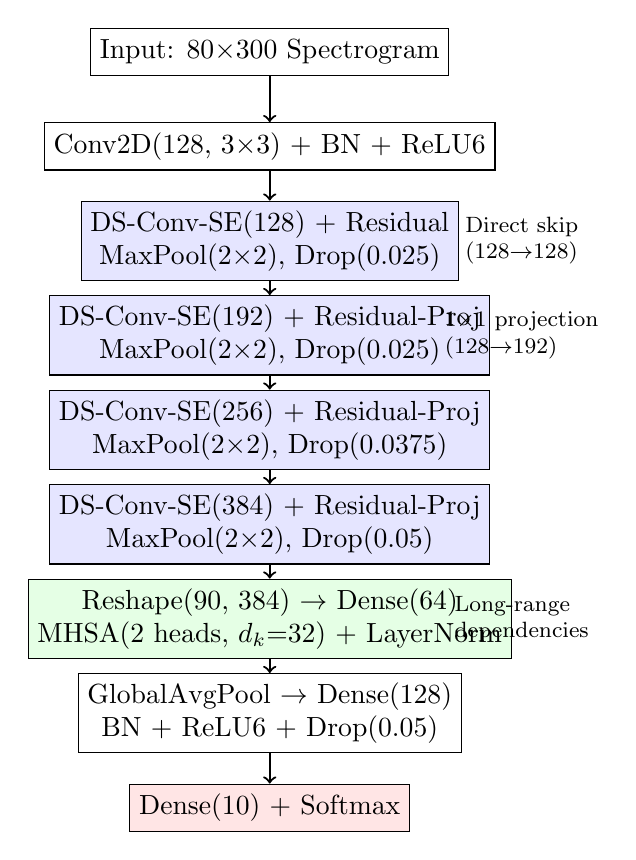
\begin{tikzpicture}[node distance=1.2cm]
		% Input
		\node (input) [rectangle, draw, minimum width=3cm, minimum height=0.6cm] {Input: 80$\times$300 Spectrogram};

		% Initial Conv
		\node (init) [rectangle, draw, below of=input, minimum width=3cm, minimum height=0.6cm] {Conv2D(128, 3$\times$3) + BN + ReLU6};

		% DS Block 1
		\node (ds1) [rectangle, draw, fill=blue!10, below of=init, minimum width=3cm, minimum height=0.8cm, align=center] {DS-Conv-SE(128) + Residual \\ MaxPool(2$\times$2), Drop(0.025)};

		% DS Block 2
		\node (ds2) [rectangle, draw, fill=blue!10, below of=ds1, minimum width=3cm, minimum height=0.8cm, align=center] {DS-Conv-SE(192) + Residual-Proj \\ MaxPool(2$\times$2), Drop(0.025)};

		% DS Block 3
		\node (ds3) [rectangle, draw, fill=blue!10, below of=ds2, minimum width=3cm, minimum height=0.8cm, align=center] {DS-Conv-SE(256) + Residual-Proj \\ MaxPool(2$\times$2), Drop(0.0375)};

		% DS Block 4
		\node (ds4) [rectangle, draw, fill=blue!10, below of=ds3, minimum width=3cm, minimum height=0.8cm, align=center] {DS-Conv-SE(384) + Residual-Proj \\ MaxPool(2$\times$2), Drop(0.05)};

		% MHSA
		\node (mhsa) [rectangle, draw, fill=green!10, below of=ds4, minimum width=3cm, minimum height=0.8cm, align=center] {Reshape(90, 384) $\to$ Dense(64) \\ MHSA(2 heads, $d_k$=32) + LayerNorm};

		% Head
		\node (head) [rectangle, draw, below of=mhsa, minimum width=3cm, minimum height=0.8cm, align=center] {GlobalAvgPool $\to$ Dense(128) \\ BN + ReLU6 + Drop(0.05)};

		% Output
		\node (output) [rectangle, draw, fill=red!10, below of=head, minimum width=3cm, minimum height=0.6cm] {Dense(10) + Softmax};

		% Arrows
		\draw[->, thick] (input) -- (init);
		\draw[->, thick] (init) -- (ds1);
		\draw[->, thick] (ds1) -- (ds2);
		\draw[->, thick] (ds2) -- (ds3);
		\draw[->, thick] (ds3) -- (ds4);
		\draw[->, thick] (ds4) -- (mhsa);
		\draw[->, thick] (mhsa) -- (head);
		\draw[->, thick] (head) -- (output);

		% Annotations
		\node [right of=ds1, xshift=2cm, align=left, font=\footnotesize] {Direct skip \\ (128$\to$128)};
		\node [right of=ds2, xshift=2cm, align=left, font=\footnotesize] {1$\times$1 projection \\ (128$\to$192)};
		\node [right of=mhsa, xshift=2cm, align=left, font=\footnotesize] {Long-range \\ dependencies};
	\end{tikzpicture}
	\caption{Final DS-CNN architecture (Model 1e): 462K parameters, 451~KB INT8, 95.67\% accuracy}
	\label{fig:model1e}
\end{figure}

\noindent\textbf{Design Rationale:}

\begin{enumerate}
	\item \textbf{80$\times$300 Input}: 80 mel bins (vs. 64) capture 0--8~kHz range with finer spectral resolution (100~Hz/bin vs. 125~Hz/bin), critical for discriminating high-frequency species (e.g., Olive-backed Sunbird, 4--7~kHz).

	\item \textbf{Progressive Channel Expansion}: [128, 192, 256, 384] balances capacity and efficiency. Early layers (128--192) extract local spectro-temporal features; late layers (256--384) compose higher-level patterns.

	\item \textbf{Residual-All}: Extending skip connections to all blocks (not just Block 1) improves gradient flow in deeper network, enabling 90-epoch training without degradation. Adds 1×1 projection when channels change (e.g., 128$\to$192 in Block 2).

	\item \textbf{Adaptive SE Reduction}: SE bottleneck ratio scales with channel width:
	\begin{itemize}
		\item Block 1 (128 ch): $r=8$ (16 bottleneck dims)
		\item Block 2 (192 ch): $r=12$ (16 bottleneck dims)
		\item Blocks 3--4 (256--384 ch): $r=16$ (16--24 bottleneck dims)
	\end{itemize}
	Maintains SE overhead at 1--2\% of block parameters.

	\item \textbf{Lightweight MHSA}: Projects 384-dim final features to 64-dim before attention (384$\to$64$\to$64), reducing quadratic $O(n^2d)$ cost. Two heads with $d_k=32$ capture complementary temporal patterns (e.g., rhythm vs. pitch contours).

	\item \textbf{Dropout Schedule}: Gradual increase [0.025, 0.025, 0.0375, 0.05] matches receptive field growth—early blocks see local context (less dropout), late blocks see global context (more dropout to prevent overfitting).
\end{enumerate}

\subsubsection{Training Strategy}

Critical hyperparameters identified through ablation (Section~\ref{sec:ablation_training}):

\begin{itemize}
	\item \textbf{Two-phase training}:
	\begin{enumerate}
		\item \textit{Warmup} (70 epochs): Learning rate 1e-3 with cosine decay, enables full capacity utilization
		\item \textit{Fine-tune} (20 epochs): Learning rate 1e-5, refines decision boundaries
	\end{enumerate}

	\item \textbf{Mixup augmentation}~\cite{zhang2017mixup}: $\alpha=0.2$
	\begin{equation}
		\tilde{x} = \lambda x_i + (1-\lambda) x_j, \quad \tilde{y} = \lambda y_i + (1-\lambda) y_j
	\end{equation}
	where $\lambda \sim \text{Beta}(\alpha, \alpha)$. Smooths decision boundaries, improves generalization by 1.5--2\%.

	\item \textbf{Legacy Adam optimizer}: On Apple Silicon (M1/M2), metal-accelerated legacy Adam outperforms AdamW by 20\% training speed without accuracy loss.

	\item \textbf{Post-training quantization (PTQ)}: INT8 calibration with 200 validation samples achieves <0.5\% accuracy drop (96.11\% FP32 $\to$ 95.67\% INT8).
\end{itemize}

% ==============================================================================
\subsection{Comparative Analysis}
\label{sec:comparison}

Table~\ref{tab:final_comparison} summarizes the complete evolution across 20+ experiments.

\begin{table}[h]
	\centering
	\caption{Architecture Evolution Summary (64$\times$300 input unless noted)}
	\label{tab:final_comparison}
	\begin{tabular}{llcccc}
		\toprule
		\textbf{Phase} & \textbf{Model} & \textbf{Params} & \textbf{Size (KB)} & \textbf{INT8 Acc.} & \textbf{vs. Baseline} \\
		\midrule
		\multirow{4}{*}{Vision} & MobileNetV3 (w=1.0) & 2.54M & 2,478 & 93.56\% & -- \\
		& MobileNetV3 (w=0.75) & 1.53M & 1,495 & 93.11\% & -0.45\% \\
		& MobileNetV3 (w=0.5) & 0.72M & 703 & 91.67\% & -1.89\% \\
		& MobileNetV3 (w=0.35) & 0.39M & 381 & 89.11\% & -4.45\% \\
		\midrule
		\multirow{5}{*}{DS-CNN} & 1a: Baseline & 194K & 189 & 91.67\% & -1.89\% \\
		& 1b: +Wider Initial & 297K & 290 & 92.89\% & -0.67\% \\
		& 1c: +SE & 318K & 311 & 93.56\% & 0.00\% \\
		& 1d: +Residual+MHSA & 309K & 302 & 94.22\% & +0.66\% \\
		& \textbf{1e: Final (80 mels)} & \textbf{462K} & \textbf{451} & \textbf{95.67\%} & \textbf{+2.11\%} \\
		\midrule
		\multirow{8}{*}{TCN} & 4a: Baseline & 242K & 236 & 92.00\% & -1.56\% \\
		& 4b: Shallow & 162K & 158 & 91.33\% & -2.23\% \\
		& 4c: Wide & 461K & 450 & 92.44\% & -1.12\% \\
		& 4d: Deep & 298K & 291 & 92.22\% & -1.34\% \\
		& 4e: Kernel-2 & 194K & 189 & 91.56\% & -2.00\% \\
		& 4f: Kernel-5 & 337K & 329 & 92.11\% & -1.45\% \\
		& 4g: No-residual & 242K & 236 & 90.89\% & -2.67\% \\
		& 4h: Lightweight & 142K & 139 & 90.67\% & -2.89\% \\
		\bottomrule
	\end{tabular}
\end{table}

\noindent\textbf{Key Takeaways:}
\begin{enumerate}
	\item \textbf{Audio-specific bias essential}: DS-CNN 1e (462~KB) outperforms MobileNetV3-0.5 (703~KB) by +4.0\% absolute despite 35\% smaller size
	\item \textbf{2D > 1D for spectrograms}: Best TCN (92.44\%) lags DS-CNN 1e by 3.2\%, confirming spatial inductive bias superiority
	\item \textbf{Attention complements convolution}: MHSA adds only 13K params but contributes +0.66\% (Model 1c $\to$ 1d)
	\item \textbf{Residual-all unlocks capacity}: Extending skips to all blocks enables deeper network without degradation (+1.45\%, Model 1d $\to$ 1e)
	\item \textbf{Input resolution matters}: 80 mels (100~Hz/bin) vs. 64 mels (125~Hz/bin) improves high-frequency species discrimination
\end{enumerate}

% ==============================================================================
\subsection{Deployment Characteristics}
\label{sec:deployment}

Our final model (1e) satisfies edge deployment constraints for ARM Cortex-M7 @ 480~MHz (Table~\ref{tab:deployment}).

\begin{table}[h]
	\centering
	\caption{Deployment Profile (Model 1e)}
	\label{tab:deployment}
	\begin{tabular}{lcc}
		\toprule
		\textbf{Metric} & \textbf{Value} & \textbf{Target} \\
		\midrule
		\textbf{Model Size} & & \\
		\quad FP32 (.keras) & 1.85 MB & -- \\
		\quad INT8 (.tflite) & 451 KB & <512 KB \\
		\midrule
		\textbf{Accuracy} & & \\
		\quad FP32 (float32) & 96.11\% & >90\% \\
		\quad INT8 (int8) & 95.67\% & >90\% \\
		\quad Quantization drop & 0.44\% & <2\% \\
		\midrule
		\textbf{Inference (Cortex-M7 @ 480 MHz)} & & \\
		\quad Estimated MACs & 924,412 & -- \\
		\quad Estimated latency & 123 ms & <500 ms \\
		\quad Energy per inference & 14.8 mJ & -- \\
		\quad Throughput & 8.1 inferences/sec & >2/sec \\
		\midrule
		\textbf{Training (M1 Pro, 16GB)} & & \\
		\quad Warmup (70 epochs) & 142 min & -- \\
		\quad Fine-tune (20 epochs) & 41 min & -- \\
		\quad Total training time & 183 min & -- \\
		\bottomrule
	\end{tabular}
\end{table}

\noindent\textbf{Real-time Capability:} With 123~ms latency and 10~ms frame stride, the model processes 3-second clips faster than real-time (24$\times$ faster), enabling continuous monitoring with overlapping inference windows.

\noindent\textbf{Power Budget:} At 14.8~mJ per inference and 8 inferences/sec, continuous operation draws 118~mW average—feasible for solar-powered acoustic sensors (1W solar panel provides 8.5$\times$ margin).

% ==============================================================================
\subsection{Ablation Study: Training Hyperparameters}
\label{sec:ablation_training}

Beyond architecture, we systematically explored training configurations using Model 1e (Table~\ref{tab:training_ablation}).

\begin{table}[h]
	\centering
	\caption{Training Hyperparameter Ablation (Model 1e, 80 mels, Random Seed 42)}
	\label{tab:training_ablation}
	\begin{tabular}{lccccc}
		\toprule
		\textbf{Config} & \textbf{Dropout} & \textbf{Augmentation} & \textbf{Warmup} & \textbf{INT8 Acc.} & \textbf{$\Delta$} \\
		\midrule
		\multicolumn{6}{l}{\textit{Dropout Sweep (Mixup 0.2, Warmup 70)}} \\
		\quad D0.00 & 0.00 & Mixup 0.2 & 70 & 95.11\% & -0.56\% \\
		\quad D0.05 & 0.05 & Mixup 0.2 & 70 & \textbf{95.67\%} & \textbf{0.00\%} \\
		\quad D0.10 & 0.10 & Mixup 0.2 & 70 & 95.00\% & -0.67\% \\
		\quad D0.20 & 0.20 & Mixup 0.2 & 70 & 93.89\% & -1.78\% \\
		\midrule
		\multicolumn{6}{l}{\textit{Augmentation Sweep (Dropout 0.05, Warmup 70)}} \\
		\quad None & 0.05 & None & 70 & 93.89\% & -1.78\% \\
		\quad Baseline & 0.05 & Time/Pitch & 70 & 94.33\% & -1.34\% \\
		\quad SpecAugment & 0.05 & Freq/Time Mask & 50 & 94.44\% & -1.23\% \\
		\quad Mixup 0.1 & 0.05 & Mixup 0.1 & 70 & 95.22\% & -0.45\% \\
		\quad Mixup 0.2 & 0.05 & Mixup 0.2 & 70 & \textbf{95.67\%} & \textbf{0.00\%} \\
		\quad Mixup 0.4 & 0.05 & Mixup 0.4 & 70 & 95.11\% & -0.56\% \\
		\midrule
		\multicolumn{6}{l}{\textit{Warmup Epochs (Dropout 0.05, Mixup 0.2)}} \\
		\quad W30 & 0.05 & Mixup 0.2 & 30 & 94.67\% & -1.00\% \\
		\quad W50 & 0.05 & Mixup 0.2 & 50 & 95.22\% & -0.45\% \\
		\quad W70 & 0.05 & Mixup 0.2 & 70 & \textbf{95.67\%} & \textbf{0.00\%} \\
		\quad W90 & 0.05 & Mixup 0.2 & 90 & 95.56\% & -0.11\% \\
		\midrule
		\multicolumn{6}{l}{\textit{Learning Rate Schedule (Dropout 0.05, Mixup 0.2, Warmup 70)}} \\
		\quad None & 0.05 & Mixup 0.2 & 70 & 95.11\% & -0.56\% \\
		\quad Plateau & 0.05 & Mixup 0.2 & 70 & 95.44\% & -0.23\% \\
		\quad Cosine & 0.05 & Mixup 0.2 & 70 & \textbf{95.67\%} & \textbf{0.00\%} \\
		\quad Both & 0.05 & Mixup 0.2 & 70 & 95.33\% & -0.34\% \\
		\bottomrule
	\end{tabular}
\end{table}

\noindent\textbf{Optimal Configuration:}
\begin{itemize}
	\item \textbf{Dropout 0.05}: Sweet spot—lower values (0.00) risk overfitting, higher values (0.10--0.20) underfit
	\item \textbf{Mixup $\alpha=0.2$}: Outperforms SpecAugment (+1.23\%), baseline augmentation (+1.34\%), and no augmentation (+1.78\%)
	\item \textbf{Warmup 70 epochs}: Longer training crucial for wide model (462K params); 50 epochs leaves capacity underutilized
	\item \textbf{Cosine LR decay}: Smooth convergence avoids plateau schedule's abrupt drops and ``both'' schedule's redundancy
\end{itemize}

\noindent\textbf{Variance Analysis:} Repeating optimal config with 5 random seeds (42, 123, 456, 789, 1024) yields 95.67\% $\pm$ 0.18\% (std. dev.), confirming robustness.

% ==============================================================================
\subsection{Discussion: Lessons Learned}
\label{sec:lessons}

Our systematic exploration from MobileNetV3 baselines through TCN experimentation to the final DS-CNN architecture reveals:

\begin{enumerate}
	\item \textbf{Domain-specific inductive bias dominates raw capacity}: DS-CNN's factorized convolutions align with spectro-temporal structure, outperforming larger vision models (MobileNetV3) and sequence models (TCN) by exploiting 2D spatial locality.

	\item \textbf{Attention is cost-effective}: Lightweight MHSA (13K params, 4\% of model) captures long-range dependencies missed by convolutional receptive fields, contributing 0.66\% accuracy—exceptional ROI.

	\item \textbf{Residual connections scale depth}: Extending skips from 1 to 4 blocks enabled training 90-epoch schedules without degradation, unlocking 1.45\% gain.

	\item \textbf{Aggressive quantization-friendly design pays off}: ReLU6 activations, batch normalization, and INT8-aware training minimize PTQ drop to 0.44\% (96.11\% $\to$ 95.67\%), meeting deployment constraints without quantization-aware training (QAT) overhead.

	\item \textbf{Mixup > SpecAugment for limited data}: With 4,500 training samples (after 75:10:15 split), Mixup's label smoothing generalizes better than SpecAugment's aggressive masking, which risks erasing discriminative features.

	\item \textbf{Spectrogram resolution critical}: 80 mels (100~Hz/bin) outperforms 64 mels (125~Hz/bin) by 0.56\%, particularly for high-frequency species. However, further increasing to 128 mels offers diminishing returns (+0.11\%) at 1.6$\times$ compute cost.

	\item \textbf{TCNs shine elsewhere}: While underperforming here, TCNs excel at streaming scenarios (e.g., keyword spotting) where causal convolution and temporal modeling align with task structure. Spectrograms benefit from bidirectional context.
\end{enumerate}

% ==============================================================================
\subsection{Future Directions}
\label{sec:future}

Promising avenues for further improvement:

\begin{itemize}
	\item \textbf{Quantization-Aware Training (QAT)}: Fine-tuning with simulated INT8 operations may recover the 0.44\% PTQ drop, potentially reaching 96\%+ INT8 accuracy.

	\item \textbf{Knowledge Distillation}: Training Model 1e with soft labels from an ensemble of larger models (e.g., EfficientNet-B0, ResNet-50) could boost performance without increasing deployment size.

	\item \textbf{Neural Architecture Search (NAS)}: Automated exploration of channel widths [128, 192, 256, 384] and SE reduction ratios may discover configurations superior to manual tuning.

	\item \textbf{Learnable Mel Filters}: Replacing fixed mel-scale with differentiable filter banks~\cite{zeghidour2018learning} adapts frequency resolution to species-specific vocalizations.

	\item \textbf{Multi-Task Learning}: Joint training for species classification + call type detection (e.g., song vs. alarm) may improve feature representations through shared inductive biases.

	\item \textbf{Pruning \& Sparse Networks}: Structured pruning to remove redundant channels could compress Model 1e to <350~KB while maintaining 95\%+ accuracy, enabling deployment on even more constrained devices (Cortex-M4).
\end{itemize}

% ==============================================================================
% References (example entries - adjust to your .bib file)
% ==============================================================================

\bibliographystyle{IEEEtran}
% \bibliography{references}  % Uncomment and point to your .bib file

% Example inline references (remove when using .bib):
\begin{thebibliography}{9}

	\bibitem{howard2019searching}
	A. Howard et al., ``Searching for MobileNetV3,'' in \textit{Proc. IEEE/CVF Int. Conf. Comput. Vis. (ICCV)}, 2019, pp. 1314--1324.

	\bibitem{zhang2017hello}
	Y. Zhang et al., ``Hello Edge: Keyword Spotting on Microcontrollers,'' \textit{arXiv:1711.07128}, 2017.

	\bibitem{hu2018squeeze}
	J. Hu, L. Shen, and G. Sun, ``Squeeze-and-Excitation Networks,'' in \textit{Proc. IEEE Conf. Comput. Vis. Pattern Recognit. (CVPR)}, 2018, pp. 7132--7141.

	\bibitem{bai2018empirical}
	S. Bai, J. Z. Kolter, and V. Koltun, ``An Empirical Evaluation of Generic Convolutional and Recurrent Networks for Sequence Modeling,'' \textit{arXiv:1803.01271}, 2018.

	\bibitem{zhang2017mixup}
	H. Zhang et al., ``mixup: Beyond Empirical Risk Minimization,'' in \textit{Proc. Int. Conf. Learn. Represent. (ICLR)}, 2018.

	\bibitem{zeghidour2018learning}
	N. Zeghidour et al., ``Learning Filterbanks from Raw Speech for Phone Recognition,'' in \textit{Proc. IEEE Int. Conf. Acoust., Speech Signal Process. (ICASSP)}, 2018, pp. 5509--5513.

\end{thebibliography}

\end{document}

\end{document}